\documentclass[11pt, openright]{book}

    % Cover Variables
	\newcommand{\ctitle}{Base de Données}
        \newcommand{\cautor}{Lucas Lescure}
		\newcommand{\ctoptitle}{TP RCP30}

    % Header Variables
        \newcommand{\headRE}{\emph{\thepage}}
        \newcommand{\headLE}{\emph{\thesection. \rightmark}}
        \newcommand{\footRE}{}
        \newcommand{\footLE}{}

    % TOC Variables
        \newcommand{\toctitle}{Table of Content}
        \newcommand{\tocchapter}{Chapter}
        \newcommand{\toccount}{3}
  
    % Chapter Variables
        \newcommand{\chvar}{Chapter -}

\usepackage[a4paper, total={16cm, 22.125cm}]{geometry}

% Page Style
\usepackage[]{environ}
% Cover Page 
\usepackage{tikz}
\makeatletter
\def\parsecomma#1,#2\endparsecomma{\def\page@x{#1}\def\page@y{#2}}
\tikzdeclarecoordinatesystem{page}{
    \parsecomma#1\endparsecomma
    \pgfpointanchor{current page}{north east}
    % Save the upper right corner
    \pgf@xc=\pgf@x%
    \pgf@yc=\pgf@y%
    % save the lower left corner
    \pgfpointanchor{current page}{south west}
    \pgf@xb=\pgf@x%
    \pgf@yb=\pgf@y%
    % Transform to the correct placement
    \pgfmathparse{(\pgf@xc-\pgf@xb)/2.*\page@x+(\pgf@xc+\pgf@xb)/2.}
    \expandafter\pgf@x\expandafter=\pgfmathresult pt
    \pgfmathparse{(\pgf@yc-\pgf@yb)/2.*\page@y+(\pgf@yc+\pgf@yb)/2.}
    \expandafter\pgf@y\expandafter=\pgfmathresult pt
}
\makeatother


% Object formatting
\usepackage[12pt]{moresize}
\usepackage[]{anyfontsize}
\usepackage{titlesec}
\usepackage{import}
\usepackage{floatrow}
\usepackage{enumitem}
\usepackage{changepage}
\usepackage[normalem]{ulem}
\usepackage{array}
\newcommand{\ul}[1]{\underline{#1}}

\usepackage[]{chngcntr}
\usepackage{ifthen}
\ifthenelse{\figcountdepth > 1}
  {\counterwithin{figure}{section}\counterwithin{table}{section}}
  {}

\usepackage[format=plain, labelfont=it, textfont=it]{caption}
\makeatletter
\def\@makecaption#1#2{%
    \vskip\abovecaptionskip
    \sbox\@tempboxa{\textit{#1.} #2}

       
   

    \ifdim \wd\@tempboxa >\hsize
        #1. #2\par
    \else
        \global \@minipagefalse
        \hb@xt@\hsize{\hfil\box\@tempboxa\hfil}
    \fi
    \vskip\belowcaptionskip}
\makeatother

\DeclareCaptionFormat{underline}{\uline{#1#2#3}\par}

% Sections
\titleformat{\section}{\fontsize{16}{19.2}\bfseries}{\thesection.}{0.25em}{}
\titleformat{\subsection}{\fontsize{14}{16.8}\bfseries}{\tab\thesubsection.}{0.25em}{}
\titleformat{\subsubsection}{\fontsize{10}{12}}{\uline{\thesubsubsection)\enspace}}{0em}{\uline}





% Geometry

% Typewritting

\setlength{\parskip}{1em}
\setlength{\parindent}{0em}


\newenvironment{items}[3][0pt]
{\def\closesep{#3}
    \vspace{#2}
    \begin{itemize}
        \setlength{\itemsep}{#1}
        \setlength{\topsep}{0pt}
        \setlength{\partopsep}{0pt}}
        {\end{itemize}
    \vspace{\closesep}}

\newenvironment{enum}[3][0pt]
{\defclosesep{#3}
    \vspace{#2}
    \begin{enumerate}
        \setlength{\itemsep}{#1}
        \setlength{\topsep}{0pt}
        \setlength{\partopsep}{0pt}}
        {\end{enumerate}
    \vspace{\closesep}}

\newenvironment{eq}[2]
{\def\closesep{#2}
    \vspace{#1}
    \begin{align*}}
        {\end{align*}
    \vspace{\closesep}}

\newenvironment{lfeq}[2]
{\def\closesep{#2}
    \vspace{#1}
    \begin{flalign*}}
        {\end{flalign*}
    \vspace{\closesep}}
% List Formatting


\NewEnviron{dent}[1]{
    \vspace{-10pt}
    \begin{adjustwidth}{7mm}{}
        \uline{#1}\hspace{2mm}
        \BODY
    \end{adjustwidth}
    \vspace{-10pt}
}


\usepackage[framemethod=tikz]{mdframed}
\newcounter{count_theorem}[section]\setcounter{count_theorem}{0}
\newcommand{\thetheorem}{\arabic{count_theorem}}

\newcounter{count_exercise}[section]\setcounter{count_exercise}{0}
\newcommand{\theexercise}{\arabic{count_exercise}}


\newenvironment{theorem}[1][]{
    \refstepcounter{count_theorem}
    \mdfsetup{
        linecolor=red!30,
        innerbottommargin=10pt,
        linewidth=2pt,
        topline=false,
        bottomline=false,
        rightline=false,
        shadow=true,
        shadowsize=4.5pt,
        frametitlerule=false,
        apptotikzsetting={
                \tikzset{
                    mdfbackground/.append style={
                            left color=red!8,right color=red!3
                        }
                }
            }
    }
    \begin{mdframed}[]\relax
        \ifstrempty{#1}
        {\textbf{Theorem~\thetheorem.} }
        {\textbf{Theorem~\thetheorem.~#1} }
        }
        {\end{mdframed}\vspace{-10pt}
}

\newenvironment{note}{
    \mdfsetup{innertopmargin=5pt,
        linecolor=gray!30,
        linewidth=2pt,
        topline=false,
        bottomline=false,
        rightline=false,
        frametitleaboveskip=0pt,
        shadow=false,
        shadowsize=4pt,
        frametitlerule=false,
        apptotikzsetting={
                \tikzset{
                    mdfbackground/.append style={
                            left color=gray!8,right color=gray!3
                        }
                }
            }
    }
    \begin{mdframed}[]\relax
        \textbf{Note. }
        }
        {\end{mdframed}\vspace{-10pt}
}

\newenvironment{example}{
    \mdfsetup{innertopmargin=5pt,
        linecolor=green!30,
        linewidth=2pt,
        topline=false,
        bottomline=false,
        rightline=false,
        frametitleaboveskip=0pt,
        shadow=false,
        shadowsize=4pt,
        frametitlerule=false,
        apptotikzsetting={
                \tikzset{
                    mdfbackground/.append style={
                            left color=green!7,right color=green!2
                        },
                    mdfframetitlebackground/.append style={
                            left color=green!7,right color=green!2
                        }
                }
            }
    }
    \begin{mdframed}[]\relax
        \textbf{Example. }
        }
        {\end{mdframed}\vspace{-10pt}
}


\usetikzlibrary{calc,arrows}

\tikzset{
    excursus arrow/.style={%
            line width=2pt,
            draw=gray!40,
            rounded corners=2ex,
        },
    excursus head/.style={
            fill=white,
            font=\bfseries\sffamily,
            text=gray!80,
            anchor=base west,
        },
    excursus line/.style={%
            line width=2pt,
            draw=gray!40,
            rounded corners=2ex,
        }
}

\newenvironment{exercise}[1][]{%
    \refstepcounter{count_exercise}
    \mdfsetup{
        singleextra={
                \path let \p1=(P), \p2=(O) in (\x2,\y1) coordinate (Q);
                \path let \p1=(Q), \p2=(O) in (\x1,{(\y1-\y2)/2}) coordinate (M);
                \path [excursus line] ($(O)+(5em,0ex)$) -| (M) |- ($(Q)+(20em,0ex)$);
                \node [excursus head] at ($(Q)+(2.5em,-0.75pt)$) {\ifstrempty{#1}{Exercise \theexercise}{Exercise \theexercise:~#1}};},
        firstextra={
                \path let \p1=(P), \p2=(O) in (\x2,\y1) coordinate (Q);
                \path [excursus arrow,-to] (O) |- ($(Q)+(12em,0ex)$) .. controls +(0:16em) and +(185:6em) .. ++(23em,2ex);},
        middlelinewidth=2.5em,middlelinecolor=white,
        hidealllines=true,topline=true,
        innertopmargin=0.5ex,
        innerbottommargin=2.5ex,
        innerrightmargin=2pt,
        innerleftmargin=2ex,
        skipabove=0.87\baselineskip,
        skipbelow=0.62\baselineskip,
    }
    \begin{mdframed}[]\relax}
        {\end{mdframed}\vspace{-10pt}
}

% Functions and Data Plotting
\usepackage{subfig,wrapfig,adjustbox,multirow}


% Plotting Style
\usepackage{graphicx,pgfplots}
\usetikzlibrary{arrows}
\usetikzlibrary {patterns,patterns.meta}
\usepgfplotslibrary{fillbetween}
\pgfplotsset{compat=1.18}

\usepgfplotslibrary{units}
% Logarithmic Scale
\pgfplotsset{
    log x ticks with fixed point/.style={
            xticklabel={
                    \pgfkeys{/pgf/fpu=true}
                    \pgfmathparse{exp(\tick)}%
                    \pgfmathprintnumber[fixed relative, precision=3]{\pgfmathresult}
                    \pgfkeys{/pgf/fpu=false}
                }
        }
}


% Mathematics

% Formatting
\usepackage{amsmath}
\usepackage{esvect}
\usepackage{amsfonts}
\usepackage{tasks,environ}
\usepackage{xargs}
\usepackage{esint}
\usepackage[]{listings}


\usepackage[english]{babel}
\usepackage{amsthm}
%\newtheorem{theorem}{Theorem}
%\newtheorem{proof}{Proof}



%Custom Shortcuts
\newcommand{\eqi}{\Leftrightarrow}
\newcommand{\lr}[1]{\left( #1 \right)}
\newcommand{\limit}[1]{\displaystyle{\lim_{#1}}}
\newcommand{\tab}{\hspace*{7mm}}
\newcommand{\ds}[1]{\displaystyle{#1}}
\newcommand{\floor}[1]{\lfloor #1 \rfloor}
\newcommand{\R}{\mathbb{R}}
\newcommand{\N}{\mathbb{N}}
\newcommand{\Z}{\mathbb{Z}}
\newcommand{\C}{\mathbb{C}}
\newcommand{\K}{\mathbb{K}}
\newcommand{\F}{\mathcal{F}}
\newcommand{\M}{\mathcal{M}}
\renewcommand{\l}{\lambda}
\newcommand{\seg}[1]{\overline{\rm {#1}}}
\newcommand{\Int}{\int\limits}
\newcommand{\ex}{\tab \uline{Example :}\hspace{0.2cm} }
\newcommand{\vard}{\partial}
\newcommand{\Q}{\mathcal{Q}}
\newcommand{\Vect}{\operatorname{Vect}}
\newcommand{\rg}{\operatorname{rg}}
\renewcommand{\dim}{\operatorname{dim}}
\renewcommand{\Re}{\operatorname{Re}}
\renewcommand{\Im}{\operatorname{Im}}
\renewcommand{\P}{\mathcal{P}}
\newcommand{\blr}[1]{\left\{#1\right\}}
\newcommand{\linecenter}[1]{\par\vspace{2mm} \centerline{#1}\par\vspace{-2mm}}
\newcommand{\dd}{\textrm{d}}
\newcommand{\supp}{\operatorname{Supp}}
\renewcommand{\vec}{\overrightarrow}
\renewcommand{\epsilon}{\varepsilon}

% Matrix Configurations

\makeatletter
\renewcommand*\env@matrix[1][*\c@MaxMatrixCols c]{%
    \hskip -\arraycolsep
    \let\@ifnextchar\new@ifnextchar
    \array{#1}}
\makeatother


% Colors
\usepackage{xcolor}
\newcommand{\blu}{\color{blue}}
\newcommand{\Red}{\color{red}}
\newcommand{\blac}{\color{black}}

\newcommand{\red}[1]{\textcolor{red}{#1}}

\usepackage{xcolor,xspace}
\usepackage{breqn}


% Headings  
\usepackage[Glenn]{fncychap}
\ChNumVar{\fontsize{40}{42}}
\ChTitleVar{\Large\sc}
\ChNameVar{\Large\sc}
\setlength\headheight{14.5pt}
\renewcommand\FmN[1]{\chvar}



\usepackage{fancyhdr}
\usepackage{ragged2e}

% Header & Footers
\renewcommand{\chaptermark}[1]{\markboth{#1}{#1}}
\renewcommand{\sectionmark}[1]{
    \markright{ #1}
}
\pagestyle{fancy}
\fancyhf{}
\fancyhead[LE,RO]{\headLE}
\fancyhead[RE,LO]{\headRE}
\fancyfoot[LE,RO]{\footLE}
\fancyfoot[RE,LO]{\footRE}
\renewcommand{\headrulewidth}{0.5pt}
\fancyheadoffset{1cm}

\fancypagestyle{plain}{%
    \fancyhf{} % clear all header and footer fields
    \fancyfoot[LE, RO]{\footLE}
    \renewcommand{\headrulewidth}{0pt}
    \renewcommand{\footrulewidth}{0pt}}


\fancypagestyle{nohead}{%
    \fancyhf{} % clear all header 
    \fancyfoot[LE, RO]{\footLE}
    \fancyfoot[LO, RE]{\footRE}}

    \fancypagestyle{head}{%
    \fancyhf{} % clear all header 
    \fancyhead[LE,RO]{\headLE}
\fancyhead[RE,LO]{\headRE}
\renewcommand{\headrulewidth}{0.5pt}
\fancyheadoffset{1cm}
    }


\fancypagestyle{bib}{%
    \fancyhf{} % clear all header and footer fields
    \fancyhead[CE, CO]{}
    \fancyfoot[LE, RO]{\footLE}
    \fancyfoot[LO, RE]{Bibliographie}}

% Table of Contents

\renewcommand*\thechapter{\arabic{chapter}} %Usually Roman
\renewcommand*\thesection{\arabic{section}}
\renewcommand*\thesubsubsection{\thesubsection.\alph{subsubsection}}
\makeatletter
\@removefromreset{section}{chapter}
\makeatother


% Table of Contents

\usepackage{titletoc}
\usepackage{ erewhon,cabin}
\usepackage[linktoc=all]{hyperref}
\renewcommand*\contentsname{\centerline{\toctitle}}

\setcounter{secnumdepth}{3}
\setcounter{tocdepth}{\toccount}

\usepackage[subfigure]{tocloft}
\setlength\cftparskip{0pt}

\usepackage{etoolbox}
\makeatletter
\pretocmd{\chapter}{\addtocontents{toc}{\protect\addvspace{5\p@}}}{}{}
\pretocmd{\section}{\addtocontents{toc}{\protect\addvspace{-10\p@}}}{}{}
\pretocmd{\subsection}{\addtocontents{toc}{\protect\addvspace{1\p@}}}{}{}
\makeatother


% Chapter Style
\titlecontents{chapter}
[11em]
{\bigskip}
{\bfseries\textsc\tocchapter~\textsc\thecontentslabel : \textsc}
{\hspace*{-5.5em}\textbf}
{\titlerule*[1pc]{ }}[\smallskip]

% Section Style
\titlecontents{section}
[0em] % i
{\bigskip\bfseries}
{\fontsize{11}{13.2}\bfseries\uline{\thecontentslabel.\enspace}\uline}
{\hspace*{-4em}\textbf}
{\hspace{0.5pt}\uline{\hspace*{\fill}}\contentspage}

% Subsection Style
\titlecontents{subsection}
[2em] % i
{\smallskip\bfseries}
{\fontsize{10}{12}\bfseries\thecontentslabel.\enspace}
{\hspace*{-4em}}
{\titlerule*[0.5pc]{.}\contentspage}

% Subsubsection Style
\titlecontents{subsubsection}
[4em] % i
{\smallskip}
{\fontsize{10}{12}\thecontentslabel)\enspace}
{\hspace*{-4em}}
{\titlerule*[0.5pc]{.}\contentspage}










    % figure support
	\usepackage{import}
	\usepackage{xifthen}
	\pdfminorversion=7
	\usepackage{pdfpages}
	\usepackage{transparent}
	\newcommand{\incfig}[1]{%
            \def\svgwidth{\columnwidth}
            \import{./figures/}{#1.pdf_tex}
	}

	\usepackage{listings}

\definecolor{clr-background}{RGB}{255,255,255}
\definecolor{clr-text}{RGB}{0,0,0}
\definecolor{clr-string}{RGB}{200,80,21}
\definecolor{clr-namespace}{RGB}{0,0,0}
\definecolor{clr-preprocessor}{RGB}{128,128,128}
\definecolor{clr-keyword}{RGB}{0,0,255}
\definecolor{clr-type}{RGB}{0,0,200}
\definecolor{clr-variable}{RGB}{0,0,0}
\definecolor{clr-constant}{RGB}{0,100,138} % macro color
\definecolor{clr-comment}{RGB}{0,128,0}

\lstset{
        language=C++,
        backgroundcolor=\color{clr-background},
        basicstyle=\color{clr-text}\scriptsize, % any text
        stringstyle=\color{clr-string},
        identifierstyle=\color{clr-variable}, % just about anything that isn't a directive, comment, string or known type
        commentstyle=\color{clr-comment},
        % listings doesn't differentiate between types and keywords (e.g. int vs return)
        % use the user types color
        keywordstyle=\color{clr-type},
        keywordstyle={[2]\color{clr-constant}}, % you'll need to define these or use a custom language
        tabsize=4
}

	\pdfsuppresswarningpagegroup=1

\begin{document}
% Spacing
% Section Spacing
\titlespacing\section{0pt}{3pt plus 2pt minus 2pt}{6pt plus 2pt minus 1pt}
\titlespacing\subsection{0pt}{0pt plus 1pt minus 1pt}{0pt plus 3pt minus 1pt}
\titlespacing\subsubsection{0pt}{0pt plus 0pt minus 0pt}{0pt plus 2pt minus 0pt}

\usetikzlibrary{shadows}

\newgeometry{left=2.5cm, width=16cm, bottom=2.5cm, top=2.5cm}






% Cover
% Cover
\definecolor{ccolor1}{RGB}{236,145,143}
\definecolor{ccolor2}{RGB}{131,168,192}
\definecolor{ccolor3}{RGB}{182,227,150}
\definecolor{ccolor4}{RGB}{171,206,145}

\usetikzlibrary{fadings}

\begin{titlepage}
    \newgeometry{top=1cm, width=21cm, bottom=1cm}

    \begin{tikzpicture}[remember picture,overlay,every node/.style={anchor=center}]

        \coordinate (Center) at (page cs: 0,-0.5);
        %F4E Logo
        \begin{scope}[scale = 1.5]
            \foreach \angle in {0,30,...,330} {
                    \filldraw[orange!50!yellow,line width=0.01pt,shift=(Center)] (\angle:3.8637) -- (\angle+30:3.8637) -- (0,0) -- (\angle:3.8637);
                    \draw[white, line width = 7pt,shift=(Center)] (\angle:2cm) arc (\angle-60:\angle:2cm);
                    \draw[white, line width = 7pt,shift=(Center)] (\angle+30:2cm) arc (\angle+90:\angle+30:2cm);
                }
            % Outer delimiter
            \foreach \angle in {15,45,...,345} {
                    \filldraw[white, line width = 7pt,shift=(Center)] (\angle:3.8637cm) arc (\angle-15:\angle+45:2cm) arc (\angle+15:\angle-15:2cm) arc (\angle+45:\angle+15:2cm);
                }
            % Inner delimiter
            \foreach \angle in {15,45,...,345} {
                    \filldraw[white, line width = 7pt,shift=(Center)] (\angle:1.0353cm) arc (\angle-75:\angle-45:2cm) arc (\angle+75:\angle+105:2cm) -- (0,0) -- (\angle:1.0353cm);
                }
            % Stars
            \foreach \angle in {0,30,...,330} {
                    \fill[orange!50!yellow,shift=(Center)] (\angle:1.03527cm) -- ++ (231:0.175) -- ++ (33:0.35) -- ++ (177:0.35) -- ++ (321:0.35) -- ++ (105:0.35) -- ++ (249:0.35) -- ++ (33:0.35);
                }
        \end{scope}

        \node[opacity =0.07, inner sep=0pt, anchor=east] at (current page.east){
\includegraphics[width=0.5\paperwidth,height=\paperheight]{/root/.config/latex-utils/logos/invert1.png}};

        \node[opacity=0.07,inner sep=0pt, anchor=north west] at (current page.north west){
\includegraphics[width=0.5\paperwidth,height=0.5\paperheight]{/root/.config/latex-utils/logos/invert3.png}};




        \node at (page cs:0,0.345) {\Large\textsc{High School Observation and Learning Internship}};
        \node at (page cs:0,0.875) {\Large\bfseries\textsc{Observation Internship}};
        \node at (page cs:0,0.925) {\LARGE\bfseries\textsc{Lycée Français de Barcelone}};

        \node at (page cs:0.5,0) {\Large\textsc{Cyril Lescure - Pedagogical Tutor}};








        %\node[opacity=0.15, inner sep=0pt, anchor=south west] at (current page.south west){
\includegraphics[width=0.5\paperwidth,height=0.5\paperheight]{/root/.config/latex-utils/logos/invert2.png}};

        \node at (page cs:0,0.5) {\fontsize{28}{28.8}\textbf{\ctoptitle}};
        \node at (page cs:0,0.425) {\fontsize{28}{28.8}\textbf{\ctitle}};
        \draw (page cs:0.5,0.375) -- (page cs:-0.5,0.375);
        \node at (page cs:0,0.245) {\LARGE\textsc{\cautor}};
        \node at (page cs:0,0.310) {\Large\textsc{03.06.2019 - 07.06.2019}};


    \end{tikzpicture}
\end{titlepage}


\newgeometry{width=18.625cm, bottom=2cm, top=2cm}

\tikz[remember picture, overlay] \node[opacity=0.3,inner sep=0pt, anchor=north east] at (current page.north east){
\includegraphics[angle=-90,origin=c,width=0.5\paperheight,height=0.5\paperwidth]{/root/.config/latex-utils/logos/invert3.png}};
\tikz[remember picture,overlay] \node[opacity=0.3,inner sep=0pt, anchor=south east] at (current page.south east){
\includegraphics[angle=90,width=0.5\paperwidth,height=0.5\paperheight]{/root/.config/latex-utils/logos/invert2.png}};

\tableofcontents





\newpage

\section{D'emarrage de PostgreSQL}

On récupère sous Moodle le kit \texttt{KitEtuBddPgSQL.zip} que l'on procède par extraire, ainsi que tout les fichiers \texttt{.zip} contenu à l'intérieur. \\
En ouvrant alors une fenêtre de commande on se redirige à l'emplacement de ce fichier et on renomme le répertoire \texttt{pgsql1} à \texttt{PostgreSQL\_12.4\_Portable}. Ensuite on commence par créer un nouveau \textbf{cluster} de base de donnés en modifiant le fichier \texttt{Make Cluster.bat} avec la commande suivante :
\begin{lstlisting}
		"%CD%\bin\initdb" -D "%RutaCluster%" -U postgres -W --encoding=UTF8
	\end{lstlisting}

On peut alors lancer le script dans la ligne de commande avec \texttt{"Make Cluster.bat"}. L'exécution du fichier demande un nom au répertoire du nouveau cluster. On le nommera \texttt{data2}. Une fois crée entrer le mot de passe de l'administrateur de la base de donnée.

On commence désormais par modifier les fichiers \texttt{PostgreSQL-Start.bat} \texttt{PostgreSQL-Restart.bat} \texttt{PostgreSQL-Stop.bat} en plaçant chacun des \texttt{data} en \texttt{data2}, exemple:
\begin{lstlisting}
		"%CD\bin\pg_ctl.exe%" start -D "%CD%\data2"
	\end{lstlisting}

Dans la command line on peut donc commencer le serveur SQL en tapant la commande \texttt{"PostgreSQL-Start.bat"}. Une fois initialisé on peut la modifier en utilisant le logiciel \texttt{pgAdmin}

Dans le client \texttt{pgAdmin} on crée une nouvelle connexion au serveur de façon suivante:
\begin{items}{-15pt}{-15pt}
	\item nom: PostgreSQL\_12.4\_Portable
	\item hôte: localhost
	\item port: 5432
	\item base maintenance: postgres
	\item username: postgres
	\item password: <Mot de passe>
\end{items}
Après ceci on ouvre le \texttt{Query Tool} et on crée notre serveur à partir de la commande :
\begin{lstlisting}[language=SQL]
		CREATE DATABASE plateformes_multimedia OWNER postgres ;
	\end{lstlisting}

\section{Construction de la Base de données}

\begin{figure}[ht!]
	\centering
	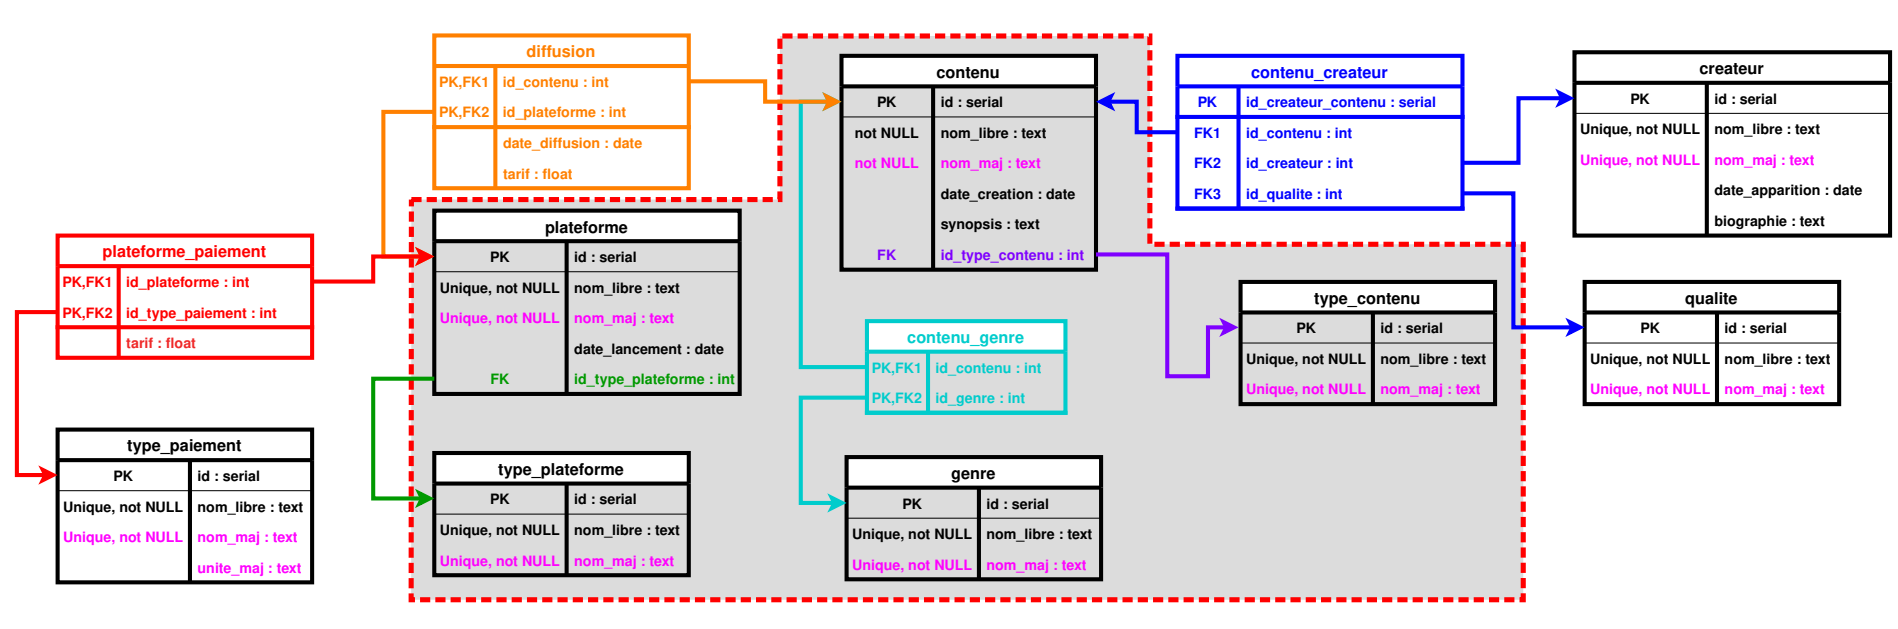
\includegraphics[width=0.95\textwidth]{./object/g1.png}
	\caption{Modèle relationnel à réaliser}
\end{figure}

\subsection{Phase 1: importation du dump dans la base de données}

Une partie est déjà crée dans le fichier \texttt{dump\_plateformes\_multimedia.sql}. C'est ce que l'on appelle un \texttt{dump}, et contient l'ensemble des requêtes SQL qui ont permis de créer et remplir une partie de la base.

On procède par ouvrir ce fichier en étant sur le \texttt{Query Tool} puis on execute (avec \texttt{F5}) . À la suite on supprime tout le code et on tape la commande:
\begin{lstlisting}
				set search_path = 'public' ;
			\end{lstlisting}

\subsection{Phase 2 : création des tables \texttt{type\_plateforme} et \texttt{contenu\_genre}}

Après l'analyse des elements on remarque qu'il manque la table \texttt{type\_plateforme} et la table tampon \texttt{contenu\_genre}. On va donc devoir les créer tout seul en respectant les contraintes associés.

Concernant la table \texttt{type\_plateforme} il faudra, une fois crée, executer le script \texttt{trigger\_insert\_update\_type\_plateforme.sql}. On devra ensuite ajouter l'attribut \texttt{id\_type\_plateforme} dans la table \texttt{plateforme} et poser la contrainte de clé étrangère vers l'\texttt{id} de \texttt{type\_plateforme}.

Pour ce qui concerne le dump, on peut ce référer à la phase 1 pour se faire.

Pour la création de la table on peut utiliser la commande suivante :
\begin{lstlisting}[language=SQL]
				CREATE TABLE type_plateforme(ID serial 	PRIMARY KEY, 
							nom_libre text UNIQUE NOT NULL,
							nom_maj text UNIQUE NOT NULL);
			\end{lstlisting}
Pour ensuite configurer la clé étrangère on doit d'abord crée l'attribut auquel appartiendra la clé étrangère pour ceci on peut ce référer au code :
\begin{lstlisting}[language=SQL]
				ALTER TABLE plateforme ADD COLUMN id_type_plateforme int;
			\end{lstlisting}
Ensuite on configure la clé étrangère avec la commande :
\begin{lstlisting}[language=SQL]
				ALTER TABLE plateforme ADD CONSTRAINT fk_id_type_plateforme
				FOREIGN KEY (id_type_plateforme) REFERENCES type_plateforme(ID)
				ON DELETE SET NULL
				ON UPDATE CASCADE;
			\end{lstlisting}
Dans lequel on référence la clé étrangère directement au tableau associé \texttt{type\_plateforme} comme il est décrit dans le modèle relationnel.

On répète ceci pour la table \texttt{contenu}.

On réalise en utilisant donc ce principe de clé la table tampon suivante:
\begin{lstlisting}[language=SQL]
				CREATE TABLE contenu_genre ()
				ALTER TABLE contenu_genre ADD COLUMN id_contenu int;
				ALTER TABLE contenu_genre ADD COLUMN id_genre int;

				ALTER TABLE contenu_genre ADD CONSTRAINT pk_contenu
				PRIMARY KEY (id_contenu, id_genre);

				ALTER TABLE contenu_genre ADD CONSTRAINT fk_id_contenu
				FOREIGN KEY (id_contenu) REFERENCES contenu(ID)
				ON DELETE CASCADE
				ON UPDATE CASCADE;

				ALTER TABLE contenu_genre ADD CONSTRAINT fk_id_genre
				FOREIGN KEY (id_genre) REFERENCES genre(ID)
				ON DELETE CASCADE
				ON UPDATE CASCADE;
			\end{lstlisting}

\subsection{Phase 3: Insertion et mise à jour de donnés}

Dans cette phase on veux pouvoir faire des requête d'insertion (INSERT INTO), de suppression(DELETE) et de mise à jour (UPDATE). \\
Avec un fichier excel, \texttt{data.xlsx} on se propose de transférer ces donnés dans notre base de donné.
Pour la copie directe de donnés, il faut sauvegarder notre excel sous format \texttt{.csv} et veillé the le codage soit en \texttt{UTF-8}. Ensuite on peut alors copier ses donnés en suivant la commande :
\begin{lstlisting}[language=SQL]
				COPY type_plateforme(ID,nom_libre)
				FROM 'D:\Users\lucas\Downloads\KitEtuBddPgSQL\KitEtuBddPgSQL' CSV
				DELIMITER ',';
			\end{lstlisting}







\end{document}
